%-=-=-=-=-=-=-=-=-=-=-=-=-=-=-=-=-=-=-=-=-=-=-=-=
%        DOCUMENT
%-=-=-=-=-=-=-=-=-=-=-=-=-=-=-=-=-=-=-=-=-=-=-=-=
\documentclass[compress,newPxFont,sthlmFooter]{beamer}
\usetheme{sthlm} %Luebeck
%\usecolortheme{sthlmv42}

%-=-=-=-=-=-=-=-=-=-=-=-=-=-=-=-=-=-=-=-=-=-=-=-=
%        PACKAGES
%-=-=-=-=-=-=-=-=-=-=-=-=-=-=-=-=-=-=-=-=-=-=-=-=
% \usepackage[backend=biber, style=numeric]{biblatex}
\usepackage{biblatex}
% \bibliographystyle{apalike}
\newcommand{\skipcite}[1]{} 

\usepackage{graphbox}
\usepackage[absolute,overlay]{textpos}
\usepackage{hyperref}
\usepackage[utf8]{inputenc}
\usepackage[english,serbian]{babel}
\usepackage{color}
\usepackage{chronology}
\renewcommand{\event}[3][e]{%
  \pgfmathsetlength\xstop{(#2-\theyearstart)*\unit}%
  \ifx #1e%
    \draw[fill=black,draw=none,opacity=0.5]%
      (\xstop, 0) circle (.2\unit)%
      node[opacity=1,rotate=45,right=.2\unit] {#3};%
  \else%
    \pgfmathsetlength\xstart{(#1-\theyearstart)*\unit}%
    \draw[fill=black,draw=none,opacity=0.5,rounded corners=.1\unit]%
      (\xstart,-.1\unit) rectangle%
      node[opacity=1,rotate=45,right=.2\unit] {#3} (\xstop,.1\unit);%
  \fi}%
  
\usepackage{amsmath}
\usepackage{amssymb,amsfonts,textcomp}
\usepackage{color}
\usepackage{placeins}
\usepackage{caption}
\usepackage{listings}
\usepackage{xcolor}
% \usepackage{droidmono}
\usepackage{subscript}

% \usecolortheme{default}
% \usefonttheme{professionalfonts}
% \usefonttheme[onlymath]{serif}

\definecolor{light_red}{RGB}{255, 100, 100}
\definecolor{light_green}{RGB}{100, 255, 100}

%-=-=-=-=-=-=-=-=-=-=-=-=-=-=-=-=-=-=-=-=-=-=-=-=
%        BEAMER OPTIONS
%-=-=-=-=-=-=-=-=-=-=-=-=-=-=-=-=-=-=-=-=-=-=-=-=
% \addbibresource{daetools.bib}

\setbeamertemplate{caption}{\insertcaption} 
\setbeamertemplate{caption label separator}{}

%\setbeameroption{show notes}
%\setbeamertemplate{note page}[plain]
%\setbeamertemplate{blocks}[rounded][shadow=true]
\definecolor{amethyst}{rgb}{0.6, 0.4, 0.8}
\definecolor{aogreen}{rgb}{0.0, 0.5, 0.0}
\definecolor{burgundy}{rgb}{0.5, 0.0, 0.13}
\definecolor{battleshipgrey}{rgb}{0.52, 0.52, 0.51}

\lstset{
    language=Python,
    basicstyle=\fontfamily{fdm}\scriptsize,
    keywordstyle=\color{blue},
    commentstyle=\color{aogreen},
    numberstyle=\color{battleshipgrey},
    stringstyle=\color{burgundy},
    identifierstyle=\color{black},
    frame=single,
    frameround=tttt,
    %numbers=left,
    keepspaces=true,
    showspaces=false,
    showtabs=false,
    showstringspaces=false,
    morekeywords={import, from, class, def, for, while, if, is, in, elif, else, not, and, or, print, break, 
                  continue, return, True, False, except, finally, import, lambda, pass, raise, try, None, __init__}
}

\lstset{
    language=C++,
    basicstyle=\fontfamily{fdm}\scriptsize,
    keywordstyle=\color{blue},
    commentstyle=\color{aogreen},
    numberstyle=\color{battleshipgrey},
    stringstyle=\color{burgundy},
    identifierstyle=\color{black},
    frame=single,
    frameround=tttt,
    %numbers=left,
    keepspaces=true,
    showspaces=false,
    showtabs=false,
    showstringspaces=false
}

\lstdefinestyle{gPROMS}{
    language=Python,
    basicstyle=\fontfamily{fdm}\scriptsize,
    keywordstyle=\color{blue},
    commentstyle=\color{aogreen},
    numberstyle=\color{battleshipgrey},
    stringstyle=\color{burgundy},
    identifierstyle=\color{black},
    frame=single,
    frameround=tttt,
    %numbers=left,
    keepspaces=true,
    showspaces=false,
    showtabs=false,
    showstringspaces=false,
    morekeywords={AS, EQUATION, PARAMETER, VARIABLE}
}

\lstdefinestyle{Modelica}{
    language=C++,
    basicstyle=\fontfamily{fdm}\scriptsize,
    keywordstyle=\color{blue},
    commentstyle=\color{aogreen},
    numberstyle=\color{battleshipgrey},
    stringstyle=\color{burgundy},
    identifierstyle=\color{black},
    frame=single,
    frameround=tttt,
    %numbers=left,
    keepspaces=true,
    showspaces=false,
    showtabs=false,
    showstringspaces=false,
    morekeywords={model, end, import, parameter, Real, equation, der}
}

% \setbeamertemplate{bibliography entry title}{}
% \setbeamertemplate{bibliography entry location}{}
% \setbeamertemplate{bibliography entry note}{}

%-=-=-=-=-=-=-=-=-=-=-=-=-=-=-=-=-=-=-=-=-=-=-=-=
%   PRESENTATION INFORMATION
%-=-=-=-=-=-=-=-=-=-=-=-=-=-=-=-=-=-=-=-=-=-=-=-=
\title{DAE Tools Software}
\subtitle{Introduction}
\author{D.D. Nikolić}
\institute
{
  DAE Tools Project, \url{http://www.daetools.com}
}
%\logo{
\includegraphics{../images/[d][a][e]_Tools_project.png}}
\date{1 April 2016} 

\hypersetup{
pdfauthor = {Dragan D. Nikolić: dnikolic@daetools.com},
pdfsubject = {},
pdfkeywords = {},
pdfmoddate= {D:\pdfdate},
pdfcreator = {}
}

% \titlegraphic{
\includegraphics{../[d][a][e]_Tools_project.png}}

% \AtBeginSection[]
% {
%   \begin{frame}
%     \frametitle{Outline}
%     \tableofcontents[currentsection]
%   \end{frame}
% }
% 
\begin{document}

% \begin{frame}
% \titlepage
% \end{frame}
\maketitle

\begin{frame}{Outline}
\tableofcontents[sectionstyle=show, 
                 subsectionstyle=hide]
\end{frame} 

\section{General Information}

\begin{frame}{What is DAE Tools?} 
Process \alert{modelling}, \alert{simulation}, and \alert{optimisation} software
\begin{itemize}
  \item Areas of application:
    \begin{itemize}
      \item Initially: chemical process industry (mass, heat and momentum transfers, chemical reactions, 
                                                  separation processes, thermodynamics, electro-chemistry)
      \item Nowadays: \alert{multi-domain}
    \end{itemize}
  \item Free/Open source software (\alert{GNU GPL})
  \item \alert{Cross-platform} (GNU/Linux, MacOS, Windows)
  \item \alert{Multiple architectures} (32/64 bit x86, ARM, ...)
\end{itemize}
\end{frame}

\begin{frame}{What is DAE Tools? (cont'd)} 
  \begin{itemize}
    \item DAE Tools \alert{is not}:
        \begin{itemize}
            \item A modelling language (such as Modelica, gPROMS, ...)
            \item An integrated software suite of data structures and routines for scientific applications (such as PETSc, Sundials, ...)
        \end{itemize}
    \item DAE Tools \alert{is}:
        \begin{itemize}
            \item A \alert{hybrid} approach between modelling and general-purpose programming languages 
            \item A higher level structure – an architectural design of interdependent software components
                  providing an API for:
                \begin{itemize}
                    \item Model development/specification
                    \item Activities on developed models (simulation, optimisation, ...)
                    \item Processing of the results
                    \item Report generation
                    \item Code generation and model exchange
                \end{itemize}
        \end{itemize}
  \end{itemize}
\end{frame}

\begin{frame}{What can be done with DAE Tools?} 
\begin{itemize}
  \item \alert{Simulation}
    \begin{itemize}
      \item Steady-State 
      \item Transient
    \end{itemize}
  \item \alert{Optimisation}
    \begin{itemize}
      \item Non-Linear Programming (NLP) problems
      \item Mixed Integer Non-Linear Programming (NLP) problems
    \end{itemize}
  \item \alert{Parameter estimation}
    \begin{itemize}
      \item Levenberg–Marquardt algorithm
    \end{itemize}
  \item \alert{Code-generation}, \alert{model-exchange}, \alert{co-simulation} 
    \begin{itemize}
      \item Modelica, gPROMS
      \item Matlab MEX-functions, Simulink user-defined S-functions
      \item Functional Mockup Interface (FMI)
      \item C99 (for embedded systems)
      \item C++ MPI (for distributed computing) 
    \end{itemize}
\end{itemize}
\end{frame}

\begin{frame}{Types of systems that can be modelled}
  \alert{Initial value problems of implicit form}, 
  (described by systems of linear, non-linear, and (partial-)differential algebraic equations).
\begin{itemize}
  \item \alert{Continuous} with some elements of \alert{event-driven} systems 
        (discontinuous equations, state transition networks and discrete events) 
  \item \alert{Steady-state} or \alert{dynamic}
  \item With \alert{lumped} or \alert{distributed} parameters 
        (finite difference, finite volume and finite element methods)
  \item Only \alert{index-1} DAE systems at the moment
\end{itemize}
\end{frame}

\section{Motivation}

\begin{frame}
\frametitle{Why modelling software?}
In general, two scenarios:
\begin{itemize}
  \item \alert{Development} of a \alert{new} product/process/...
    \begin{itemize}
        \item Reduce the time to market (TTM)
        \item Reduce the development costs (no physical prototypes)
        \item Maximise the performance, yield, productivity, purity, ...
        \item Minimise the capital and operating costs
        \item Explore the new design options in less time and no risks
    \end{itemize}

  \item \alert{Optimisation} of an \alert{existing} product/process/...
    \begin{itemize}
        \item Increase the performance, yield, productivity, purity, ...
        \item Reduce the operating costs, energy consumption, ...
        \item Debottleneck
    \end{itemize}
\end{itemize}
\end{frame}

\begin{frame}{Why \textsc{yet another} modelling software?}
Currently available options:
\begin{enumerate}
   \item \alert{Modelling languages} (domain-specific or multi-domain) 
         (Modelica \skipcite{Fritzson-and-Engelson-1998}, Ascend \skipcite{Piela-etal-1991}, gPROMS \skipcite{Barton-and-Pantelides-1994}, 
         GAMS \skipcite{Brook-etal-1988}, Dymola \skipcite{Elmqvist-1978}, APMonitor \skipcite{APMonitor-2014})
   \item \alert{General-purpose programming languages}:
      \begin{itemize}
          \item Lower level third-generation languages such as C, C++ and Fortran
                (PETSc \skipcite{petsc}, SUNDIALS \skipcite{Hindmarsh-etal-2005})
          \item Higher level fourth-generation languages such as Python (NumPy, SciPy, Assimulo \skipcite{Assimulo-2015}), Julia etc.
          \item Multi-paradigm numerical languages 
                (Matlab \skipcite{matlab}, Mathematica \skipcite{mathematica}, Maple \skipcite{maple}, 
                Scilab \skipcite{scilab}, and GNU Octave \skipcite{octave})
      \end{itemize}
 \end{enumerate}
\end{frame}

\begin{frame}{Why \textsc{yet another} modelling software? (cont'd)}
  The advantages of the \alert{Hybrid} approach over the \alert{modelling} and \alert{general-purpose} programming languages:
    \begin{enumerate}
        \item Support for the \alert{runtime model generation}
        \item Support for the \alert{runtime simulation set-up}
        \item Support for \alert{complex runtime operating procedures}
        \item \alert{Interoperability} with the \alert{$3^{rd}$ software} packages (i.e. NumPy/SciPy)
        \item Suitability for \alert{embedding} and use as a \alert{web application} or \alert{software as a service}
        \item \alert{Code-generation}, \alert{model exchange} and \alert{co-simulation} capabilities  
    \end{enumerate}
\end{frame}

\begin{frame}{Additional features}
    \begin{itemize}
        \item Support for the \alert{automatic differentiation} (ADOL-C)
        \item Support for the \alert{sensitivity analysis} through the auto-differentiation capabilities
        \item Support for the \alert{parallel} computation (OpenMP, GPGPU, MPI)
        \item Support for a large number of \alert{DAE}, \alert{LA} and \alert{NLP} solvers 
        \item Support for the generation of \alert{model reports} (XML + MathML, Latex)
        \item \alert{Export} of the \alert{simulation results} to various file formats (Matlab, Excel, json, xml, HDF5, Pandas)
    \end{itemize}
\end{frame}

\section{Programming Paradigms}

\begin{frame}{The \textsc{hybrid} approach}
  \begin{itemize}
    \item DAE Tools approach is a type of a hybrid approach:
        \begin{itemize}
            \item Applies general-purpose programming languages such as C++ and Python
        \end{itemize}
    \item But provides:
        \begin{itemize}
            \item Application Programming Interface (API) that resembles a syntax of modelling languages as much as possible
        \end{itemize}
    \item And takes advantage of the higher level languages to:
        \begin{itemize}
            \item Access the low-level functions in the operating system
            \item Access a large number of standard and third-party libraries
        \end{itemize}
  \end{itemize}
\end{frame}

\begin{frame}{The \textsc{hybrid} approach (cont'd)}
  \begin{itemize}
     \item To illustrate the \alert{hybrid} approach, consider a comparison between:
        \begin{itemize}
            \item Modelica grammar
            \item gPROMS grammar
            \item DAE Tools API    
        \end{itemize}
     \item for a very simple dynamics model:
        \begin{itemize}
            \item A cylindrical tank containing a liquid inside with an inlet and an outlet flow where 
                  the outlet flowrate depends on the liquid level in the tank
        \end{itemize}
  \end{itemize}
\end{frame}

\begin{frame}[plain]{The \textsc{hybrid} approach (\textsc{Model. lang.} vs. \textsc{DAE Tools})}
    \begin{columns}[c]
      \begin{column}{0.5\paperwidth}
        \begin{center}
          {\scriptsize \textcolor{sthlmRed}{gPROMS}:} 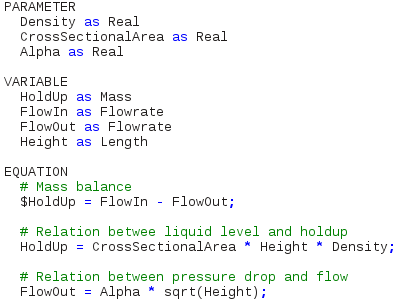
\includegraphics[align=c, width=0.32\paperwidth]{gproms_model.png}
        \end{center}
      \end{column}
      \begin{column}{0.5\paperwidth}
        \begin{center}
          {\scriptsize \textcolor{sthlmRed}{Modelica}:} 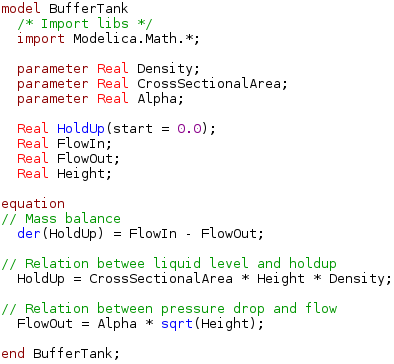
\includegraphics[align=c, width=0.32\paperwidth]{modelica_model.png}
        \end{center}
      \end{column}
    \end{columns}
    
    \begin{center}
      {\scriptsize \textcolor{sthlmRed}{DAE Tools}:} 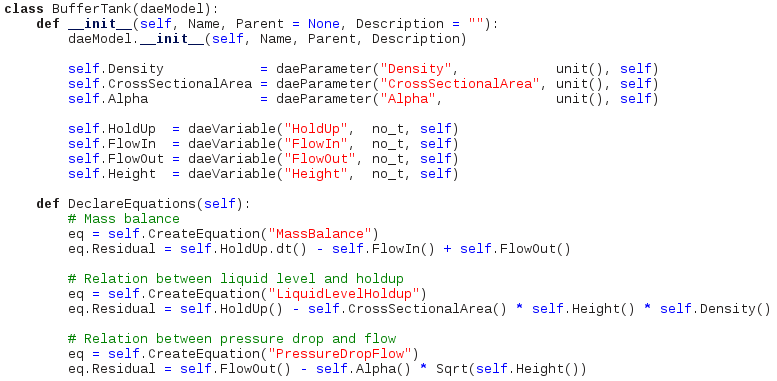
\includegraphics[align=c, width=0.6\paperwidth]{daetools_model.png}
    \end{center}
\end{frame}


\begin{frame}[plain]{The \textsc{hybrid} approach (\textsc{Model. lang.} vs. \textsc{DAE Tools})}
\tiny
{
\begin{table}
  \begin{tabularx}{\linewidth}{p{0.46\linewidth}X}
    \toprule
    \textcolor{sthlmRed}{\textbf{Modelling language approach}} & \textcolor{sthlmRed}{\textbf{DAE Tools approach}} \tabularnewline
    \midrule
    Solutions expressed in the idiom and at the level of abstraction of the problem domain
      &
    Must be emulated in the API or in some other way 
    \tabularnewline \midrule
    
    Clean and concise way of building models
      &
    Verbose and less elegant
    \tabularnewline \midrule
    
    Could be and often are simulator independent
      &
    Programming language dependent 
    \tabularnewline \midrule
    
    Cost of designing, implementing, and maintaining a language and 
    a compiler/lexical parser/interpreter
      &
    A compiler/lexical parser/interpreter is an integral part of the programming language (c++, Python) with a
    robust error handling, universal grammar and massively tested 
    \tabularnewline \midrule
    
    Cost of learning a new language vs. its limited applicability (yet another language grammar)
      &
    No learning of a new language required
    \tabularnewline \midrule
    
    Increased difficulty of integrating the DSL with other components
      &
    Calling external functions/libraries is a built-in feature 
    \tabularnewline \midrule
    
    Models usually cannot be created/modified in the runtime/on the fly (or at least not easily)
      &
    Models can be created in the runtime/on the fly and easily modified in the runtime 
    \tabularnewline \midrule
    
    Setting up a simulation is embedded in the language and it is typically difficult to do it on the fly 
    or to obtain the values from other software
      &
    Setting up a simulation is done programmaticaly and the initial values can be obtained from other software
    \tabularnewline \midrule
    
    Simulation operating procedures are not flexible
      &
    Operating procedures are completely flexible (within the limits of a programming language itself)
    \tabularnewline
    
    \bottomrule
  \end{tabularx}
\end{table}
}
\end{frame}

\begin{frame}{The \textsc{object-oriented} approach}
\begin{itemize}
  \item Everything is an \alert{object}: models, parameters, variables, equations, simulations, solvers, ... 
  \item Models, simulations, optimisations:
     \begin{itemize}
        \item Classes derived from the corresponding base classes
        \item Inherit the common functionality
        \item Perform the required functionality in overloaded functions
     \end{itemize}
  \item \alert{Hierarchical model decomposition}:
    \begin{itemize}
        \item Models can contain instances of other models
        \item Allows creation of complex, re-usable model definitions
        \item Multi-scale modelling
    \end{itemize}
  \item All C++/Python \alert{object-oriented} concepts supported, but:
    \begin{itemize}
      \item Derived classes inherit all declared DAE Tools objects  
      \item All declared DAE Tools objects are public
    \end{itemize}
\end{itemize}
\end{frame}

\begin{frame}{The \textsc{equation-oriented} (\textsc{acausal}) approach}
\begin{itemize}
  \item Equations given in an implicit form (as a residual)
    \begin{center}
      $F(\dot {x}, x, y, p) = 0$
    \end{center}
  \item Input-Output causality is not fixed:
  \begin{itemize}
    \item Increased model re-use
    \item Support for different simulation scenarios (based on a single model) by specifying different degrees of freedom
  \end{itemize}
  \item For instance, equation given in the following form:
    \begin{center}
      $x_1 + x_2 + x_3 = 0$
    \end{center}
    can be used to determine either $x_1$, $x_2$ or $x_3$ depending on what combination of variables is known:
    \begin{center}
      $x_1 = -x_2 - x_3 \; or \;  
      x_2 = -x_1 - x_3 \; or \; 
      x_3 = -x_1 - x_2$
    \end{center}
\end{itemize}
\end{frame}

\begin{frame}{Separation of the model definition from its applications}
\begin{itemize}
  \item The structure of the model (parameters, variables, equations etc.) given in the model classes ($daeModel$, $daeFiniteElementModel$) 
  \item The runtime information in the simulation class ($daeSimulation$)
  \item Single model definition, but:
  \begin{itemize}
    \item One or more different simulation scenarios
    \item One or more optimization scenarios
  \end{itemize}
\end{itemize}
\end{frame}

\section{Architecture}

\begin{frame}[plain]{The fundamental concepts/software interfaces}
\begin{columns}
    \begin{column}{0.28\paperwidth}
        \scriptsize{
        \begin{itemize}
            \item Concepts/Interfaces:
                \begin{itemize}
                    \tiny{
                        \item \textcolor{sthlmRed}{daeModel\_t}
                        \item \textcolor{sthlmRed}{daeSimulation\_t}
                        \item \textcolor{sthlmRed}{daeOptimization\_t}
                        \item \textcolor{sthlmRed}{daeBlock\_t}
                        \item \textcolor{sthlmRed}{daeDAESolver\_t}
                        \item \textcolor{sthlmRed}{daeLASolver\_t}
                        \item \textcolor{sthlmRed}{daeDataReporter\_t}
                        \item \textcolor{sthlmRed}{daeBlock\_t}
                    }
                \end{itemize}
            \item In 6 packages:
                \begin{itemize}
                \tiny{
                        \item \alert{core}
                        \item \alert{activity}
                        \item \alert{datareporting}
                        \item \alert{solvers}
                        \item \alert{logging}
                        \item \alert{units}
                    }
                \end{itemize}
        \end{itemize}
        }
     \end{column}
     
     \begin{column}{0.72\paperwidth}
         \begin{center}
             \begin{figure}
               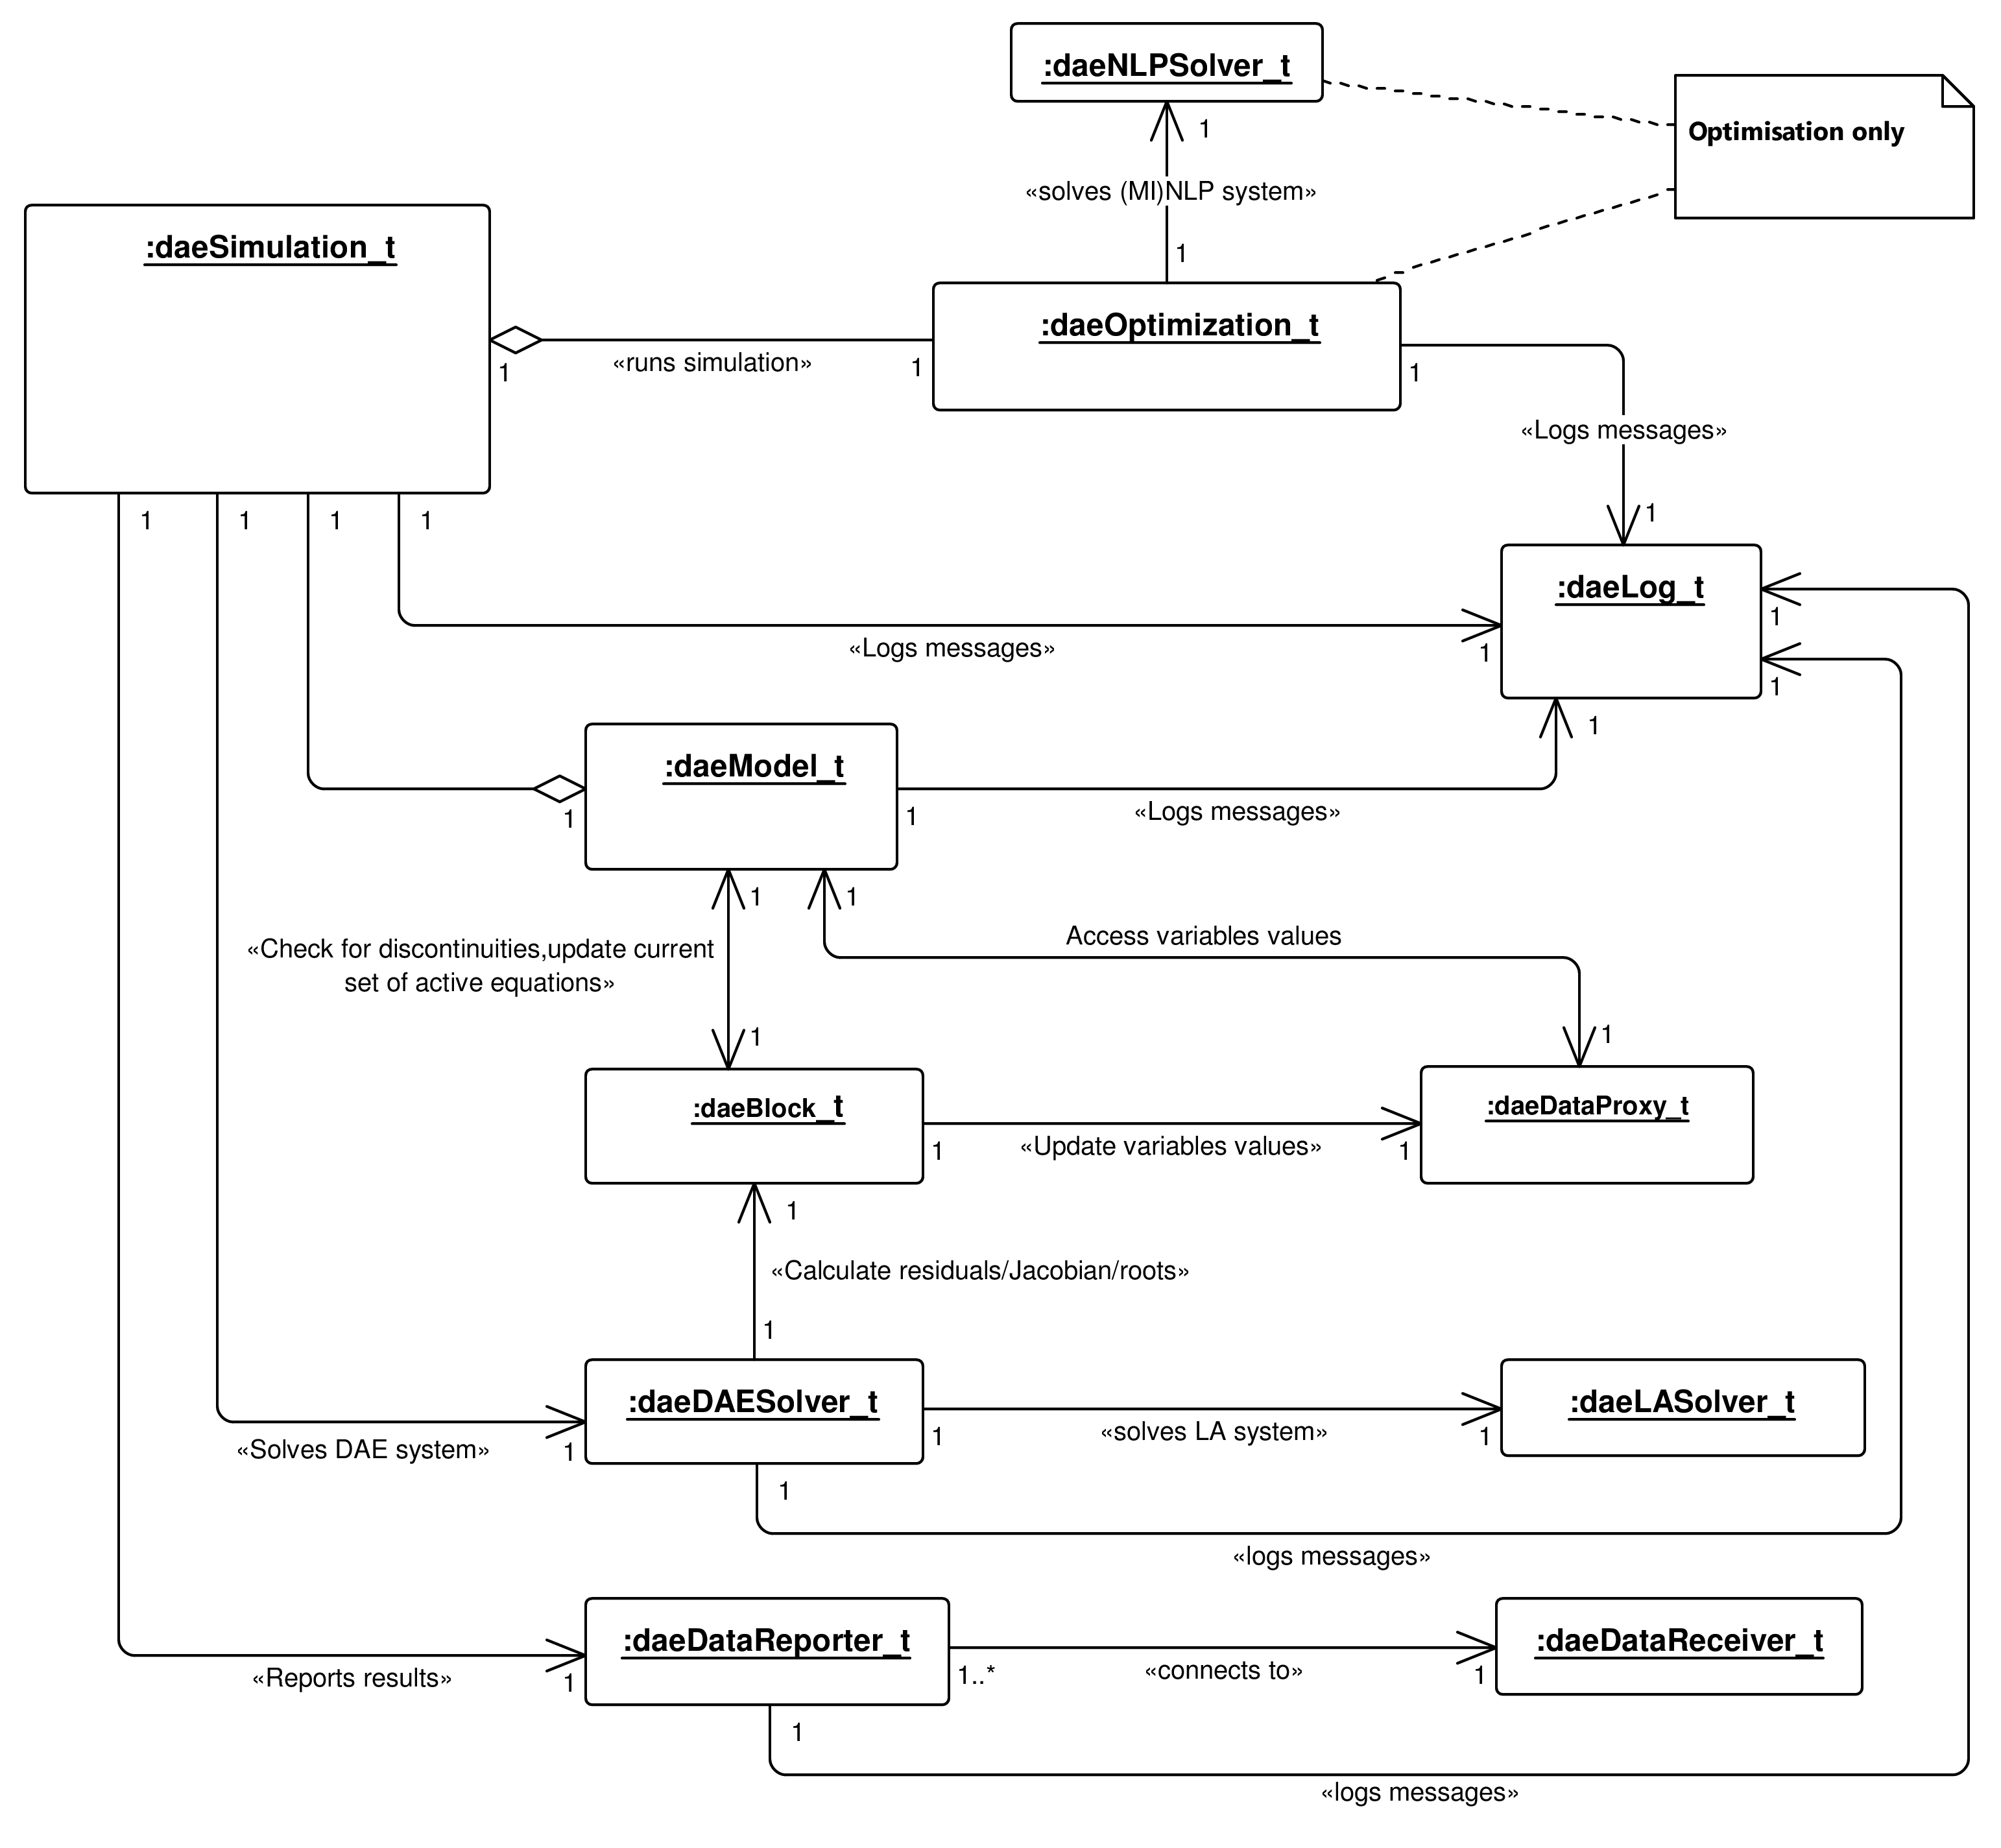
\includegraphics[width=0.68\paperwidth]{daetools-architecture.png}      
               \caption{The architecture of \alert{DAE Tools}.}
            \end{figure}
         \end{center}
     \end{column}
   \end{columns}
\end{frame}

\begin{frame}{Package \textsc{core}}
\scriptsize
{
\begin{table}
  \caption{The key modelling concepts in the \alert{core} package.}
  \begin{tabularx}{\linewidth}{l>{\raggedright}X}
    \toprule
    \textcolor{sthlmRed}{\textbf{Concept}} & \textcolor{sthlmRed}{\textbf{Description}} \tabularnewline
    \midrule
    \textcolor{sthlmRed}{\textit{daeVariableType\_t}} & Defines a variable type that has the units, lower and upper bounds, a default value and 
                                  an absolute tolerance \tabularnewline
    \textcolor{sthlmRed}{\textit{daeDomain\_t}} & Defines ordinary arrays or spatial distributions such as structured and unstructured grids \tabularnewline 
    \textcolor{sthlmRed}{\textit{daeParameter\_t}} & Defines time invariant quantities that do not change during a simulation \tabularnewline 
    \textcolor{sthlmRed}{\textit{daeVariable\_t}} & Defines time varying quantities that change during a simulation \tabularnewline 
    \textcolor{sthlmRed}{\textit{daePort\_t}} & Defines connection points between model instances for exchange of continuous quantities \tabularnewline 
    \textcolor{sthlmRed}{\textit{daeEventPort\_t}} & Defines connection points between model instances for exchange of discrete messages/events \tabularnewline
    \bottomrule
  \end{tabularx}
\end{table}
}
\end{frame}

\begin{frame}{Package \textsc{core} (cont'd)}
\scriptsize
{
\begin{table}
  \caption{The key modelling concepts in the \alert{core} package (cont'd).}
  \begin{tabularx}{\linewidth}{l>{\raggedright}X}
    \toprule
    \textcolor{sthlmRed}{\textbf{Concept}} & \textcolor{sthlmRed}{\textbf{Description}} \tabularnewline
    \midrule
    \textcolor{sthlmRed}{\textit{daePortConnection\_t}} & Defines connections between two ports \tabularnewline 
    \textcolor{sthlmRed}{\textit{daeEventPortConnection\_t}} & Defines connections between two event ports \tabularnewline
    \textcolor{sthlmRed}{\textit{daeEquation\_t}} & Defines model equations given in an implicit/acausal form \tabularnewline 
    \textcolor{sthlmRed}{\textit{daeSTN\_t}} & Defines state transition networks used to model discontinuous equations \tabularnewline
    \textcolor{sthlmRed}{\textit{daeOnConditionActions\_t}} & Defines actions to be performed when a specified condition is satisfied \tabularnewline
    \textcolor{sthlmRed}{\textit{daeOnEventActions\_t}} & Defines actions to be performed when an event is triggered on the specified event port \tabularnewline
    \textcolor{sthlmRed}{\textit{daeState\_t}} & Defines a state in a state transition network \tabularnewline 
    \textcolor{sthlmRed}{\textit{daeModel\_t}} & Represents a model \tabularnewline
    \bottomrule
  \end{tabularx}
\end{table}
}
\end{frame}

% \begin{frame}{Package core (cont'd)}
%     \begin{center}
%         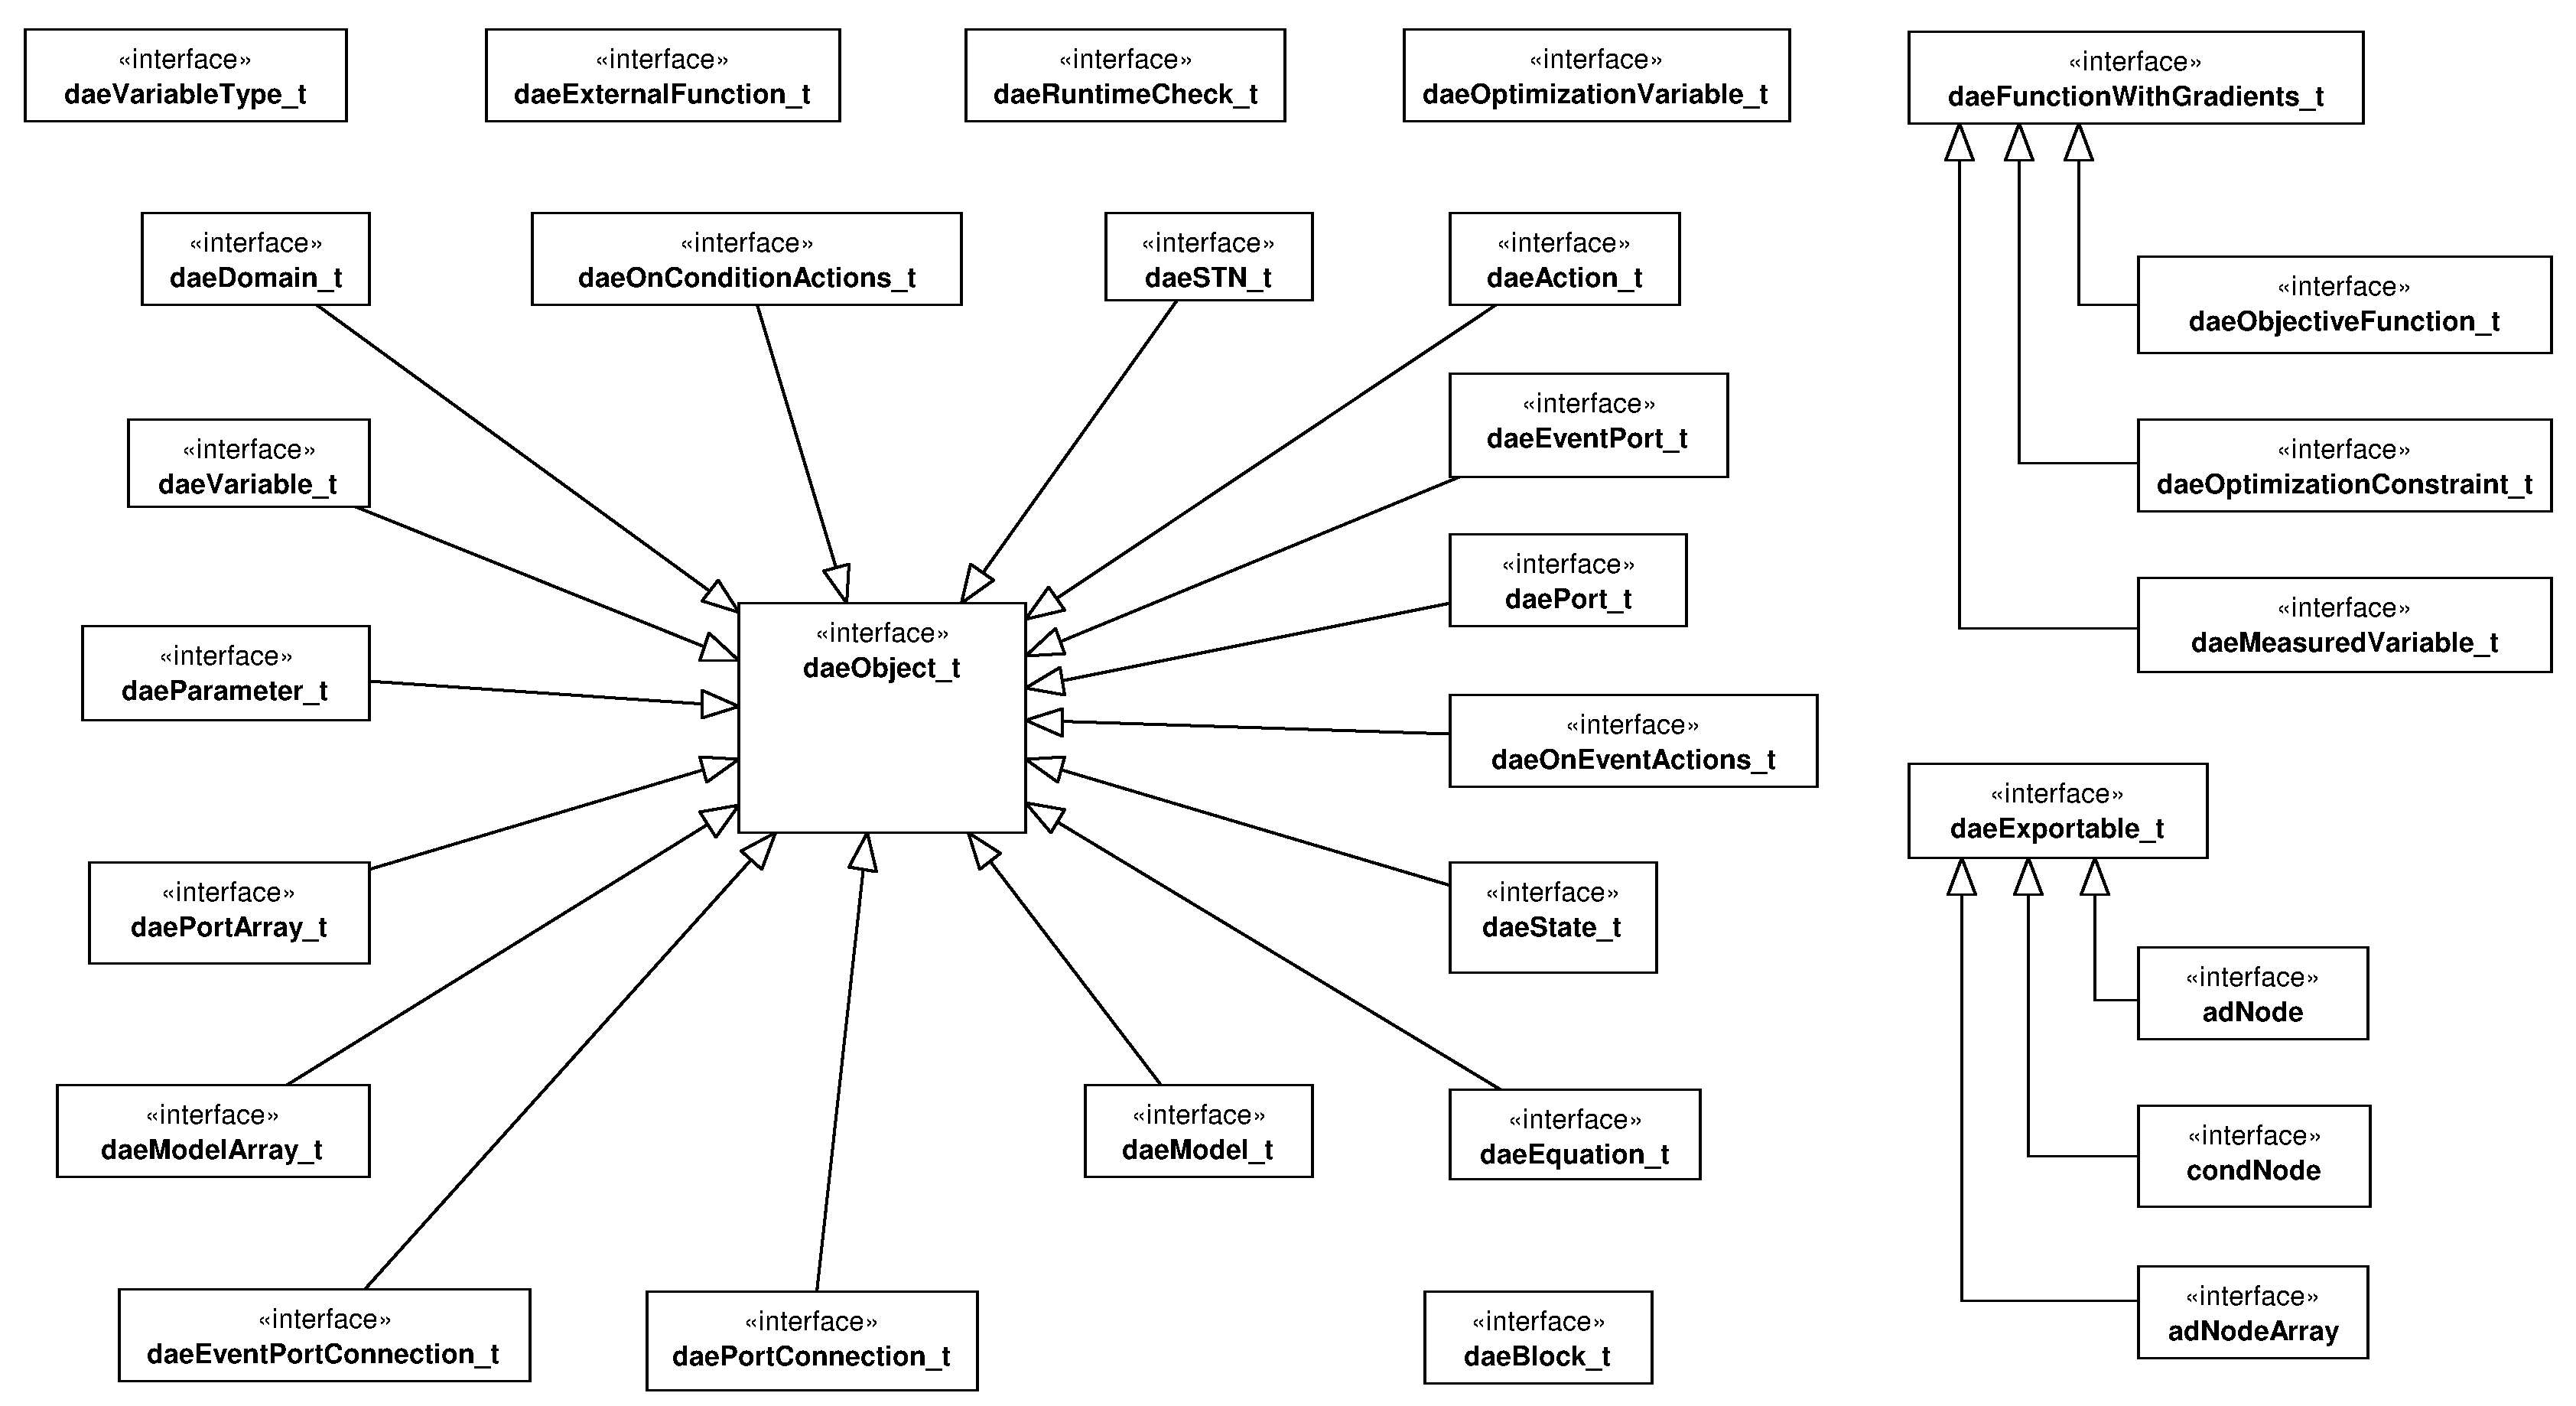
\includegraphics[width=0.9\paperwidth]{Supplemental_Figure_S1.png}      
%     \end{center}
% \end{frame}

\begin{frame}{Package \textsc{core} - interface implementations}
    \begin{center}
        \begin{figure}
            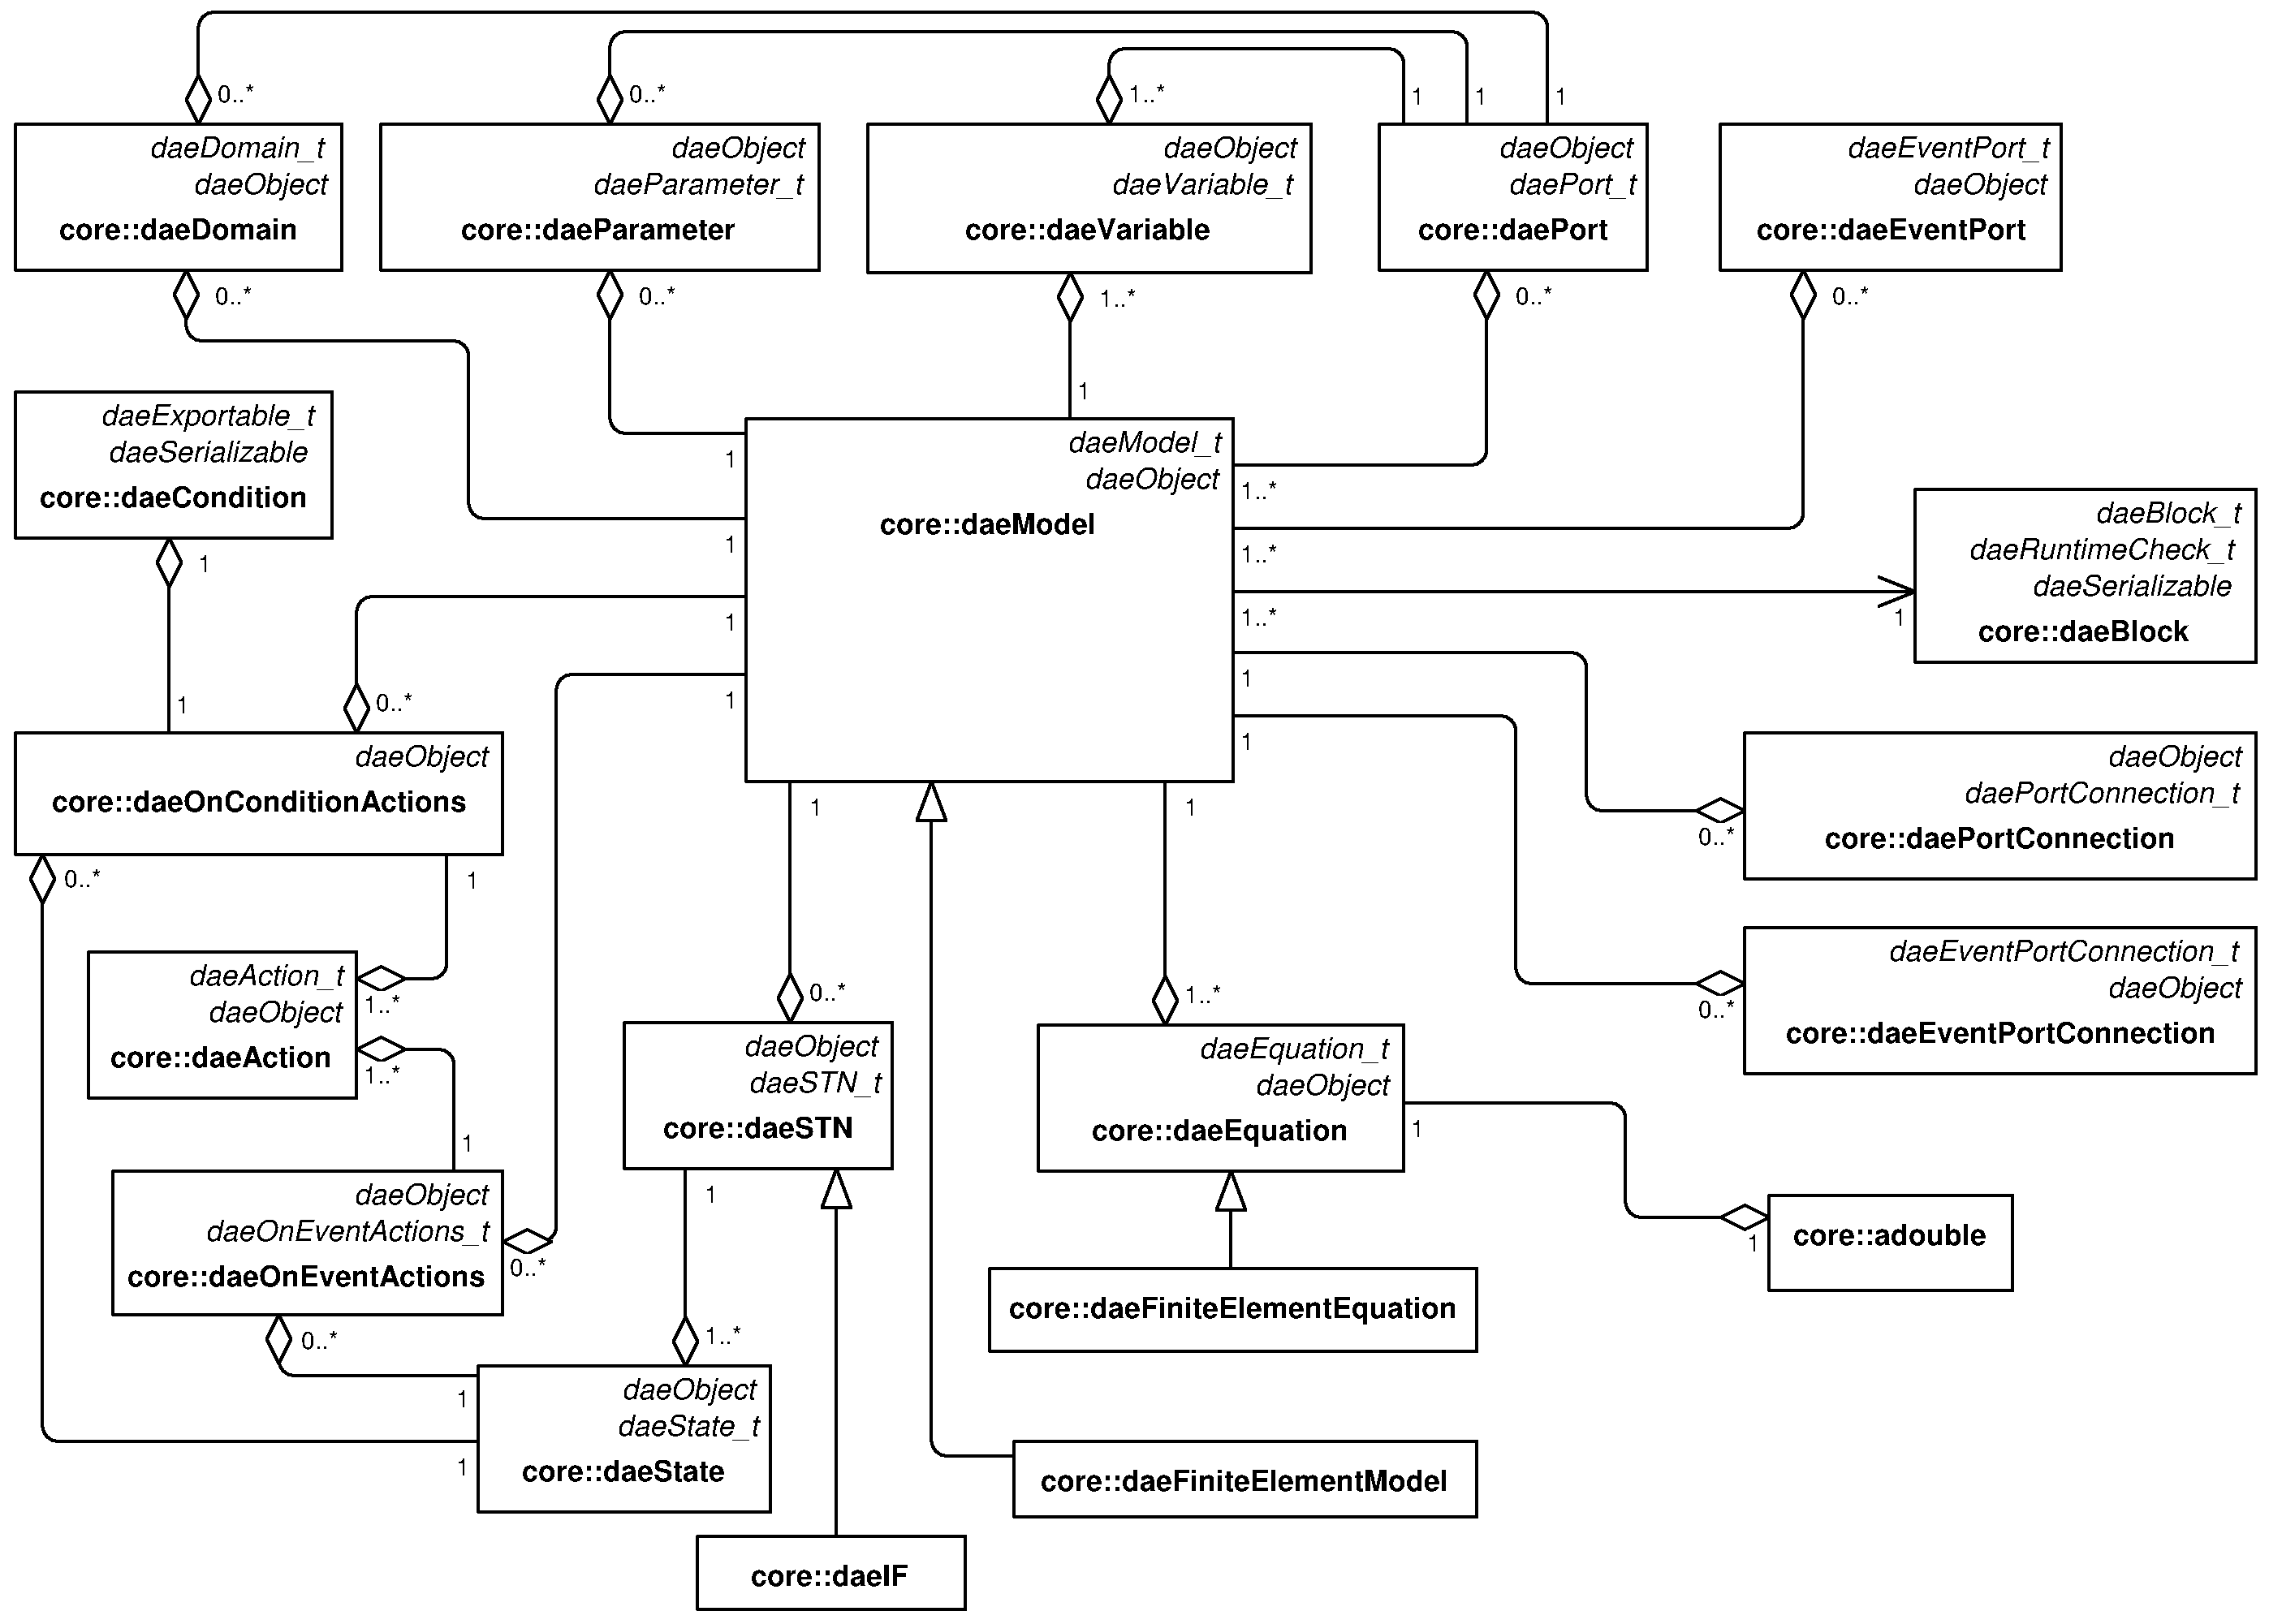
\includegraphics[width=0.8\paperwidth]{Supplemental_Figure_S3.png}      
            %\caption{\alert{core} package interface implementations.}
        \end{figure}
    \end{center}
\end{frame}

\begin{frame}{Package \textsc{activity}}
\scriptsize
{
\begin{table}
  \caption{The key concepts in the \alert{activity} package.}
  \begin{tabularx}{\linewidth}{l>{\raggedright}X}
    \toprule
    \textcolor{sthlmRed}{\textbf{Concept}} & \textcolor{sthlmRed}{\textbf{Description}} \tabularnewline
    \midrule
    \textcolor{sthlmRed}{\textit{daeSimulation\_t}} & Defines ... \tabularnewline 
    \textcolor{sthlmRed}{\textit{daeOptimisation\_t}} &  \tabularnewline
    \bottomrule
  \end{tabularx}
\end{table}
}
\end{frame}

\begin{frame}{Package \textsc{solvers}}
\scriptsize
{
\begin{table}
  \caption{The key concepts in the \alert{solvers} package.}
  \begin{tabularx}{\linewidth}{l>{\raggedright}X}
    \toprule
    \textcolor{sthlmRed}{\textbf{Concept}} & \textcolor{sthlmRed}{\textbf{Description}} \tabularnewline
    \midrule
    \textcolor{sthlmRed}{\textit{daeDAESolver\_t}} & Defines ... \tabularnewline 
    \textcolor{sthlmRed}{\textit{daeLASolver\_t}} &  \tabularnewline
    \textcolor{sthlmRed}{\textit{daeNLPSolver\_t}} &  \tabularnewline
    \textcolor{sthlmRed}{\textit{daeIDALASolver\_t}} &  \tabularnewline
    \midrule
    \textcolor{sthlmRed}{\textit{daeMatrix\_t<typename FLOAT>}} &  \tabularnewline
    \bottomrule
  \end{tabularx}
\end{table}
}
\end{frame}

\begin{frame}{Package \textsc{solvers} - interface implementations}
    \begin{center}
        \begin{figure}
            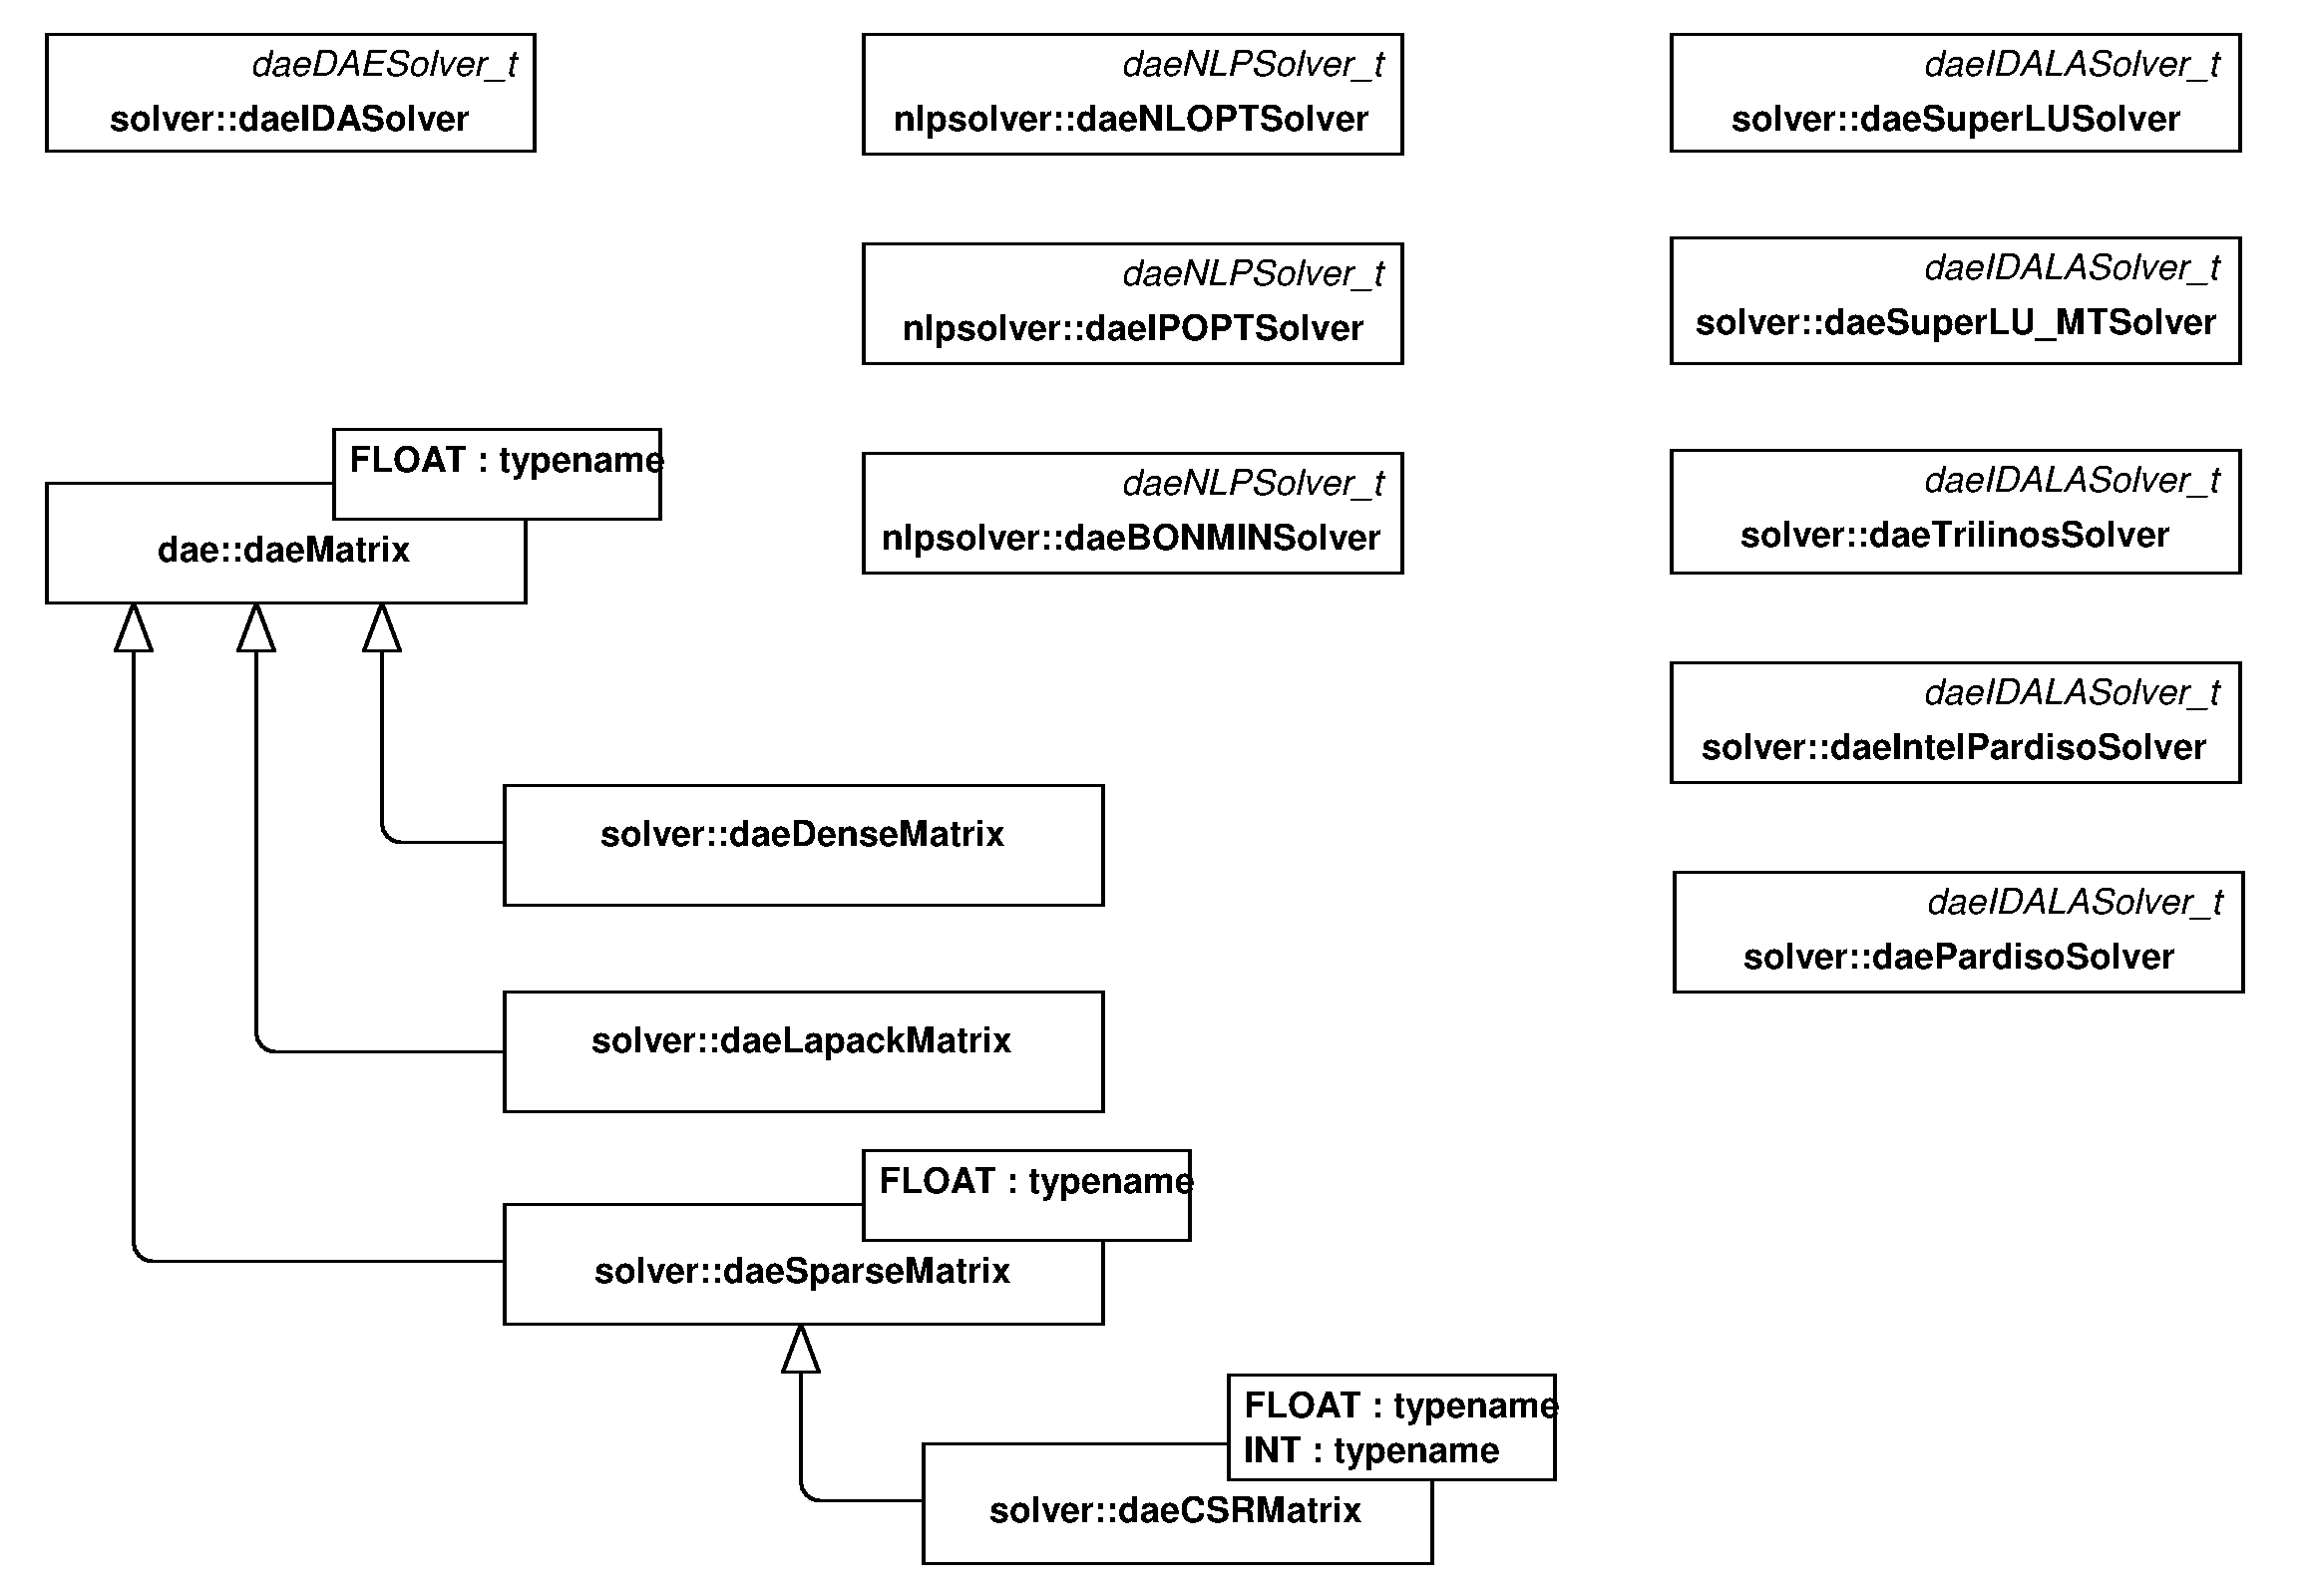
\includegraphics[width=0.75\paperwidth]{Supplemental_Figure_S5.png}      
            %\caption{\alert{solvers} package interface implementations.}
        \end{figure}
    \end{center}
\end{frame}

\begin{frame}{Package \textsc{datareporting}}
\scriptsize
{
\begin{table}
  \caption{The key concepts in the \alert{datareporting} package.}
  \begin{tabularx}{\linewidth}{l>{\raggedright}X}
    \toprule
    \textcolor{sthlmRed}{\textbf{Concept}} & \textcolor{sthlmRed}{\textbf{Description}} \tabularnewline
    \midrule
    \textcolor{sthlmRed}{\textit{daeDataReporter\_t}} & Defines ... \tabularnewline 
    \textcolor{sthlmRed}{\textit{daeDataReceiver\_t}} &  \tabularnewline
    \bottomrule
  \end{tabularx}
\end{table}
}
\end{frame}

\begin{frame}{Package \textsc{datareporting} - interface implementations}
    \begin{center}
        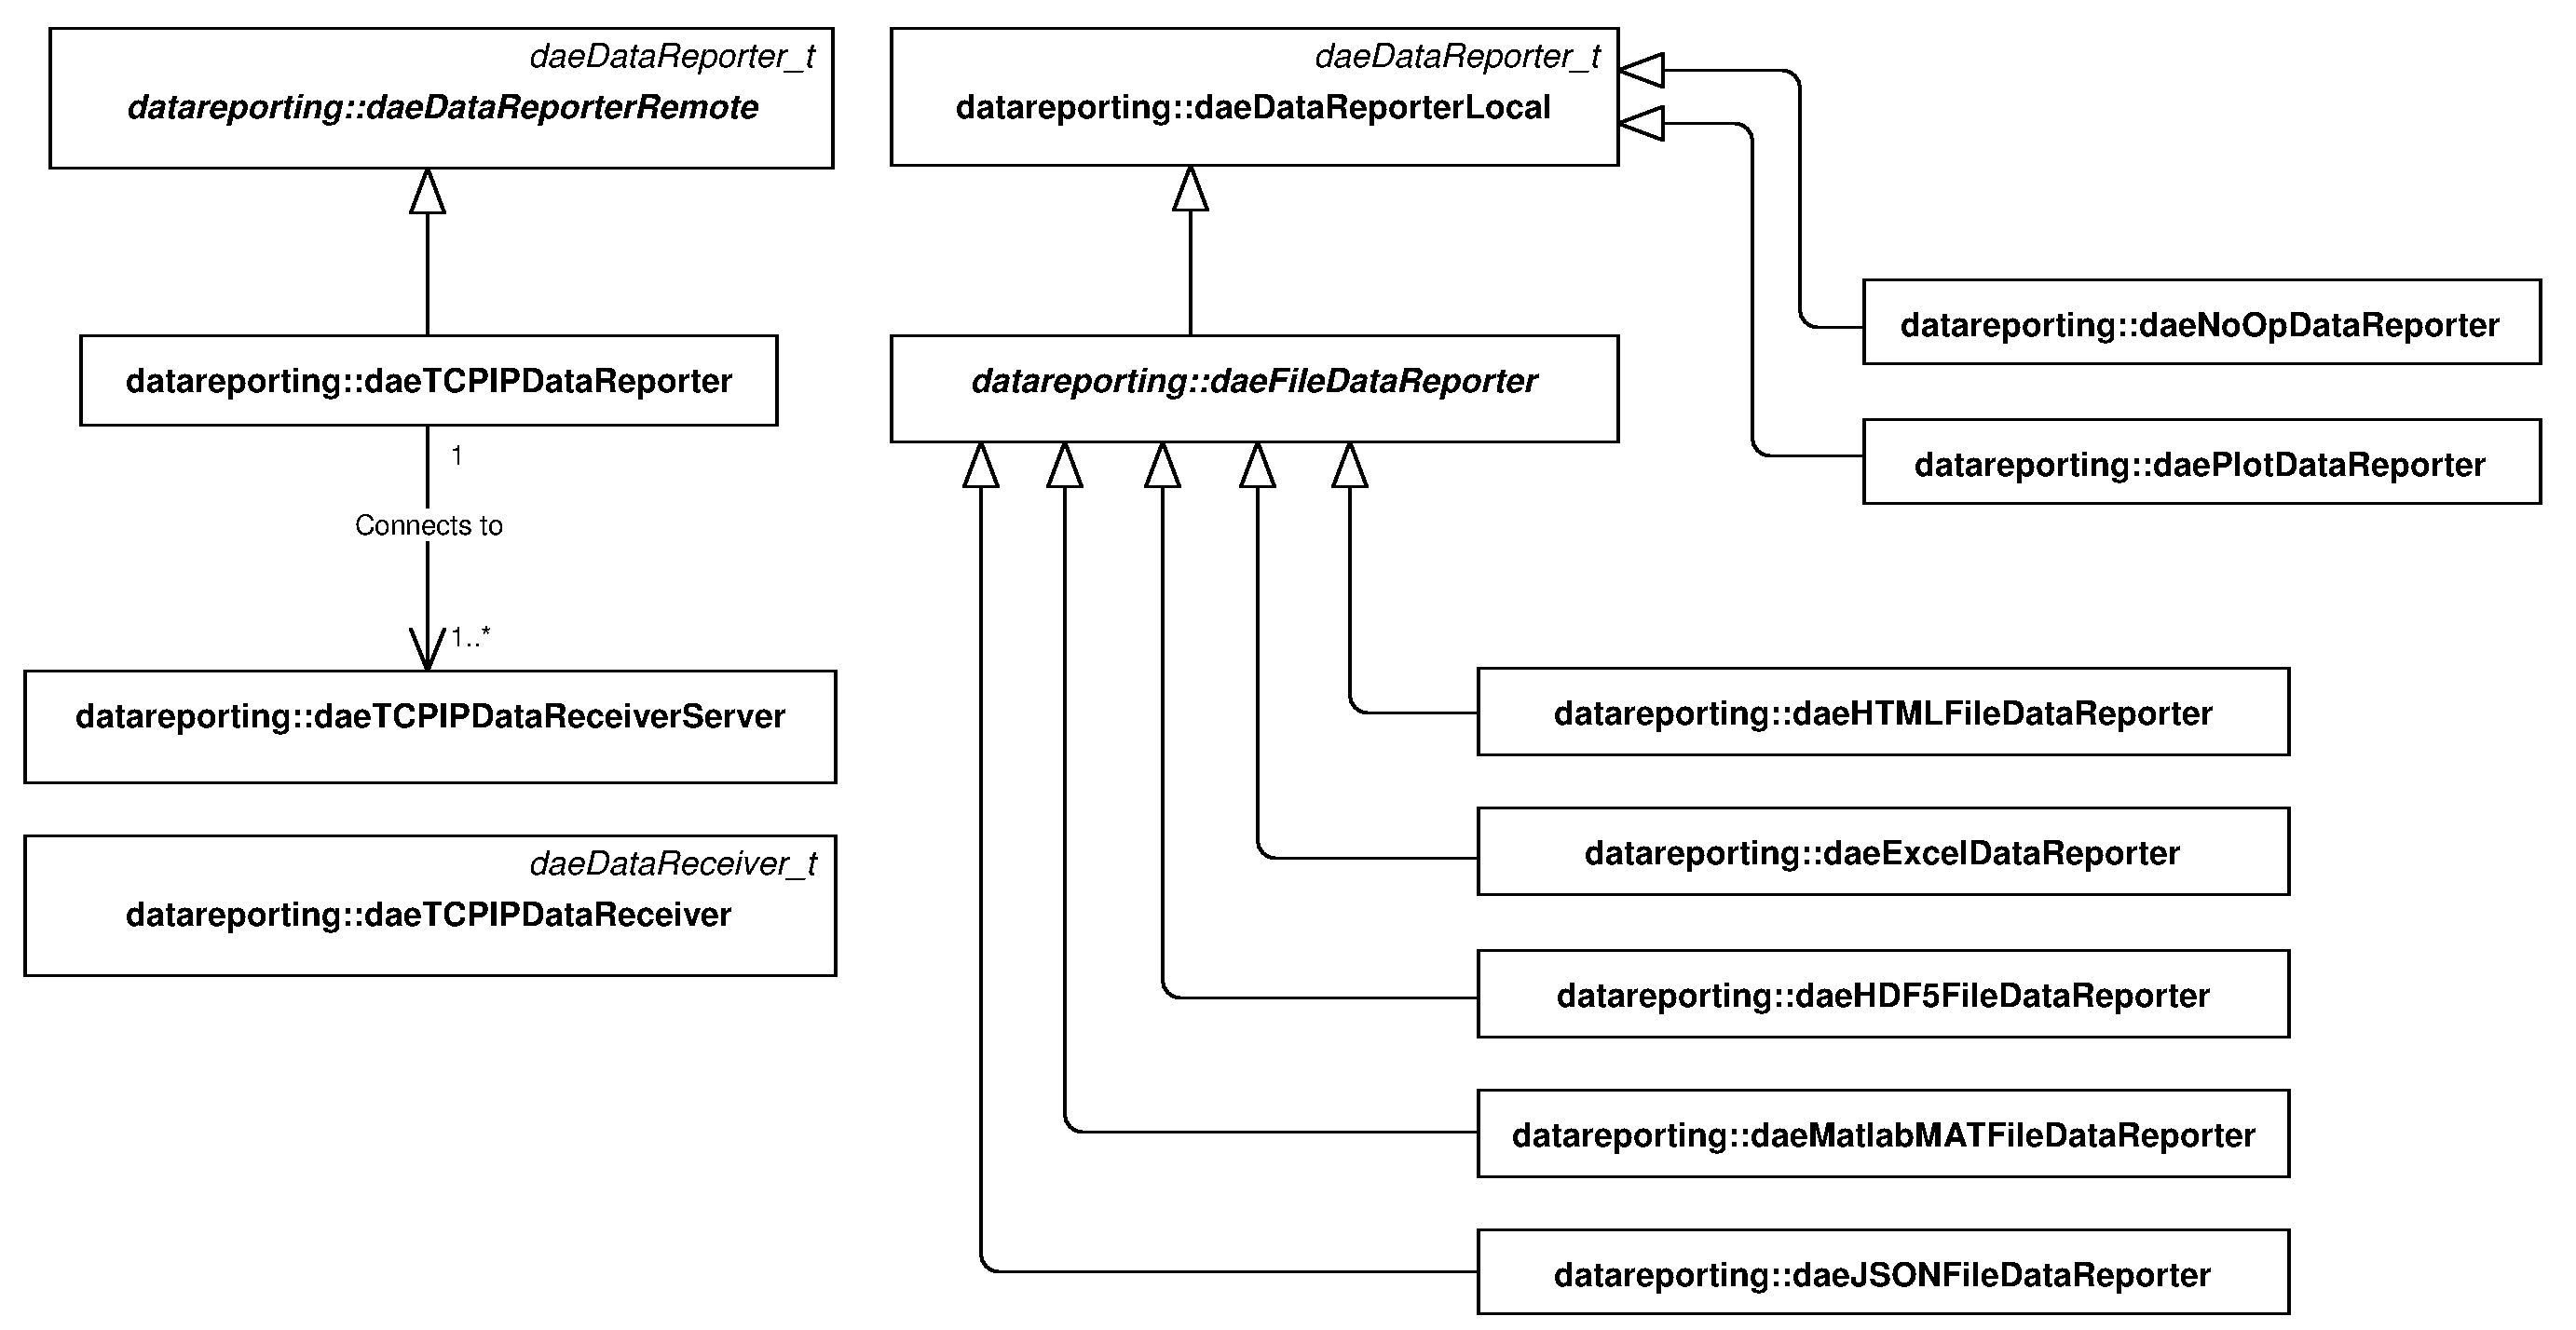
\includegraphics[width=0.8\paperwidth]{Supplemental_Figure_S6.png}      
    \end{center}
\end{frame}

\begin{frame}{Package \textsc{log} and its interface implementations}
\scriptsize
{
\begin{table}
  \caption{The key concepts in the \alert{log} package.}
  \begin{tabularx}{\linewidth}{l>{\raggedright}X}
    \toprule
    \textcolor{sthlmRed}{\textbf{Concept}} & \textcolor{sthlmRed}{\textbf{Description}} \tabularnewline
    \midrule
    \textcolor{sthlmRed}{\textit{daeLog\_t}} & Defines ... \tabularnewline 
    \bottomrule
  \end{tabularx}
\end{table}
}
    \begin{center}
        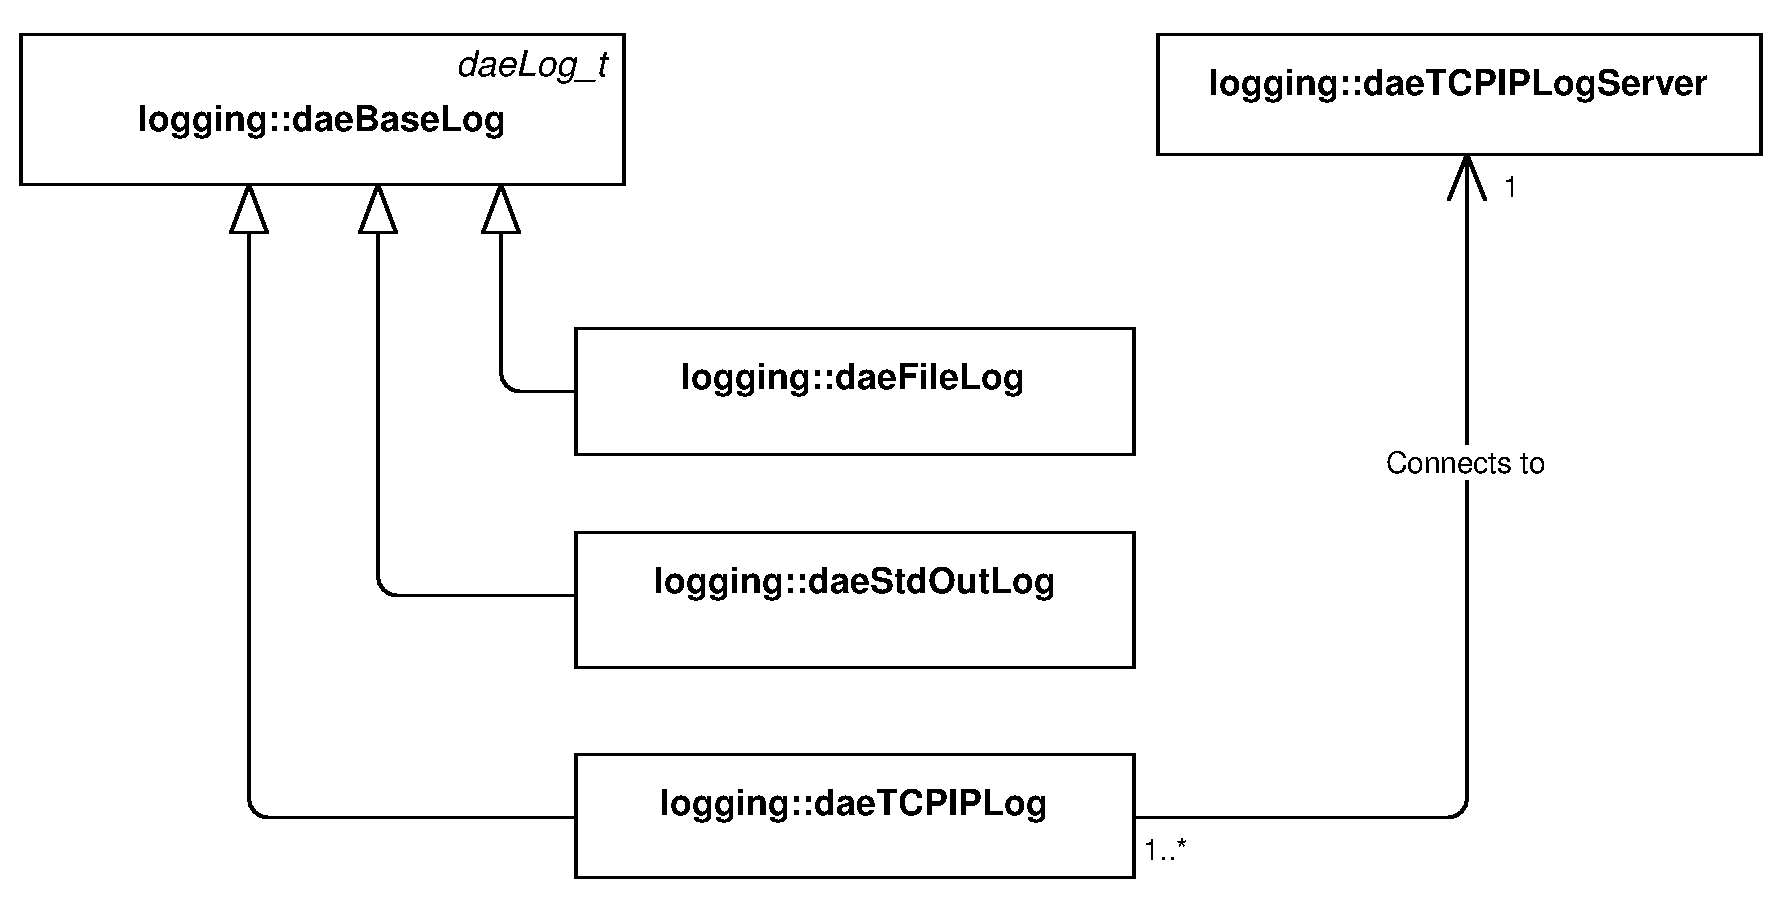
\includegraphics[width=0.6\paperwidth]{Supplemental_Figure_S7.png}      
    \end{center}
\end{frame}

\begin{frame}{Package \textsc{units}}
\scriptsize
{
\begin{table}
  \caption{The key concepts in the \alert{units} package.}
  \begin{tabularx}{\linewidth}{l>{\raggedright}X}
    \toprule
    \textcolor{sthlmRed}{\textbf{Concept}} & \textcolor{sthlmRed}{\textbf{Description}} \tabularnewline
    \midrule
    \textcolor{sthlmRed}{\textit{unit}} & Defines ... \tabularnewline 
    \textcolor{sthlmRed}{\textit{quantity}} &  \tabularnewline
    \bottomrule
  \end{tabularx}
\end{table}
}
\end{frame}

\section{Developing models with DAE Tools} 

\begin{frame}{Overview}
\end{frame}

\section{Use Cases} 

\begin{frame}{Use Case 1 - High-Level Modelling Language}
\end{frame}

\begin{frame}{Use Case 2 - Low-Level DAE Solver}
\end{frame}

\begin{frame}{Use Case 3 - Embedded Simulator (back end)}
\end{frame}

\begin{frame}{Use Case 4 - Web Application / Web Service}
\end{frame}

% \appendix
% \begin{frame}[allowframebreaks]{References}
% \begin{thebibliography}{JModelica-2010}
% 
% \bibitem[Akesson et~al., 2010]{JModelica-2010}
% Akesson, J., Arzen, K.-E., Gafvert, M., Bergdahl, T., and Tummescheit, H.
%   (2010).
% \newblock Modeling and optimization with {Optimica} and {JModelica}.org -
%   languages and tools for solving large-scale dynamic optimization problems.
% \newblock {\em Comput. Chem. Eng.}, 34(11):1737--1749.
% 
% \bibitem[Andersson et~al., 2015]{Assimulo-2015}
% Andersson, C., Fuhrer, C., and Akesson, J. (2015).
% \newblock Assimulo: A unified framework for ode solvers.
% \newblock {\em Math. Comput. Simulat.}, 116(0):26 -- 43.
% 
% \bibitem[Balay et~al., 2015]{petsc}
% Balay, S., Abhyankar, S., Adams, M.~F., Brown, J., Brune, P., Buschelman, K.,
%   Dalcin, L., Eijkhout, V., Gropp, W.~D., Kaushik, D., Knepley, M.~G., McInnes,
%   L.~C., Rupp, K., Smith, B.~F., Zampini, S., and Zhang, H. (2015).
% \newblock {PETS}c users manual.
% \newblock Technical Report ANL-95/11 - Revision 3.6, Argonne National
%   Laboratory.
% 
% \bibitem[Barton and Pantelides, 1993]{Barton-and-Pantelides-1993}
% Barton, P.~I. and Pantelides, C.~C. (1993).
% \newblock {gPROMS - A Combined Discrete/Continuous Modelling Environment for
%   Chemical Processing Systems}.
% \newblock {\em Simul. Ser.}, 25:25--34.
% 
% \bibitem[Barton and Pantelides, 1994]{Barton-and-Pantelides-1994}
% Barton, P.~I. and Pantelides, C.~C. (1994).
% \newblock {Modeling of combined discrete/continuous processes}.
% \newblock {\em AIChE J.}, 40(6):966--979.
% 
% \bibitem[Bonami et~al., 2008]{Bonami-etal-2008}
% Bonami, P., Biegler, L.~T., Conn, A.~R., Cornu{\'e}jols, G., Grossmann, I.~E.,
%   Laird, C.~D., Lee, J., Lodi, A., Margot, F., Sawaya, N., and W{\"a}chter, A.
%   (2008).
% \newblock {An algorithmic framework for convex mixed integer nonlinear
%   programs}.
% \newblock {\em Discrete Optim.}, 5(2):186--204.
% \newblock In Memory of George B. Dantzig.
% 
% \bibitem[Brook et~al., 1988]{Brook-etal-1988}
% Brook, A., Kendrick, D., and Meeraus, A. (1988).
% \newblock {GAMS, a User's Guide}.
% \newblock {\em SIGNUM Newsl.}, 23(3-4):10--11.
% 
% \bibitem[Eaton et~al., 2015]{octave}
% Eaton, J., Bateman, D., Hauberg, S., and Wehbring, R. (2015).
% \newblock {\em {GNU Octave} version 4.0.0 manual: a high-level interactive
%   language for numerical computations}.
% 
% \bibitem[Elmqvist, 1978]{Elmqvist-1978}
% Elmqvist, H. (1978).
% \newblock {\em {A Structured Model Language for Large Continuous Systems}}.
% \newblock PhD thesis, Department of Automatic Control, Lund University, Sweden.
% 
% \bibitem[Fritzson et~al., 2005]{OpenModelica-2005}
% Fritzson, P., Aronsson, P., Lundvall, H., Nystrom, K., Pop, A., Saldamli, L.,
%   and Broman, D. (2005).
% \newblock The openmodelica modeling, simulation, and development environment.
% \newblock SIMS - Scandinavian Simulation Society.
% 
% \bibitem[Fritzson and Engelson, 1998]{Fritzson-and-Engelson-1998}
% Fritzson, P. and Engelson, V. (1998).
% \newblock {Modelica --- A unified object-oriented language for system modeling
%   and simulation}.
% \newblock In Jul, E., editor, {\em {ECOOP{\rq}98 --- Object-Oriented
%   Programming}}, volume 1445 of {\em {Lecture Notes in Computer Science}},
%   pages 67--90. Springer Berlin Heidelberg.
% 
% \bibitem[Hedengren et~al., 2014]{APMonitor-2014}
% Hedengren, J.~D., Shishavan, R.~A., Powell, K.~M., and Edgar, T.~F. (2014).
% \newblock Nonlinear modeling, estimation and predictive control in apmonitor.
% \newblock {\em Comput. Chem. Eng.}, 70:133 -- 148.
% \newblock Manfred Morari Special Issue.
% 
% \bibitem[Hindmarsh et~al., 2005]{Hindmarsh-etal-2005}
% Hindmarsh, A.~C., Brown, P.~N., Grant, K.~E., Lee, S.~L., Serban, R., Shumaker,
%   D.~E., and Woodward, C.~S. (2005).
% \newblock {SUNDIALS: Suite of Nonlinear and Differential/Algebraic Equation
%   Solvers}.
% \newblock {\em ACM Trans. Math. Softw.}, 31(3):363--396.
% 
% \bibitem[Johnson, 2015]{nlopt}
% Johnson, S.~G. (2015).
% \newblock {The NLopt nonlinear-optimization package}.
% 
% \bibitem[Li, 2005]{Li-2005}
% Li, X.~S. (2005).
% \newblock {An Overview of SuperLU: Algorithms, Implementation, and User
%   Interface}.
% \newblock {\em ACM Trans. Math. Softw.}, 31(3):302--325.
% 
% \bibitem[Li et~al., 2014]{Li-etal-2014}
% Li, Y., El~Gabaly, F., Ferguson, T.~R., Smith, R.~B., Bartelt, N.~C., Sugar,
%   J.~D., Fenton, K.~R., Cogswell, D.~A., Kilcoyne, D. A.~L., Tyliszczak, T.,
%   Bazant, M.~Z., and Chueh, W.~C. (2014).
% \newblock {Current-induced transition from particle-by-particle to concurrent
%   intercalation in phase-separating battery electrodes}.
% \newblock {\em Nat. Mater.}, 13(12):1149--1156.
% 
% \bibitem[Morton, 2003]{Morton-2003}
% Morton, W. (2003).
% \newblock {Equation-Oriented Simulation and Optimization}.
% \newblock pages 317--357. Indian National Sciences Academy.
% 
% \bibitem[Piela et~al., 1991]{Piela-etal-1991}
% Piela, P.~C., Epperly, T.~G., Westerberg, K.~M., and Westerberg, A.~W. (1991).
% \newblock {ASCEND: an object-oriented computer environment for modeling and
%   analysis: The modeling language}.
% \newblock {\em Comput. Chem. Eng.}, 15(1):53--72.
% 
% \bibitem[Sala et~al., 2006]{amesos-2006}
% Sala, M., Stanley, K., and Heroux, M. (2006).
% \newblock {Amesos: A Set of General Interfaces to Sparse Direct Solver
%   Libraries}.
% \newblock In {\em {Proceedings of PARA'06 Conference, Umea, Sweden}}.
% 
% \bibitem[Schenk et~al., 2007]{Schenk-etal-2007}
% Schenk, O., W{\"a}chter, A., and Hagemann, M. (2007).
% \newblock {Matching-based preprocessing algorithms to the solution of
%   saddle-point problems in large-scale nonconvex interior-point optimization}.
% \newblock {\em Comput. Optim. Appl.}, 36(2-3):321--341.
% 
% \bibitem[{Scilab Enterprises}, 2015]{scilab}
% {Scilab Enterprises} (2015).
% \newblock {Scilab: Free and Open Source software}.
% 
% \bibitem[{The MathWorks, Inc.}, 2015]{matlab}
% {The MathWorks, Inc.} (2015).
% \newblock {MATLAB}.
% 
% \bibitem[W{\"a}chter and Biegler, 2006]{Wachter-and-Biegler-2006}
% W{\"a}chter, A. and Biegler, L.~T. (2006).
% \newblock {On the implementation of an interior-point filter line-search
%   algorithm for large-scale nonlinear programming}.
% \newblock {\em Math. Program.}, 106:25--57.
% 
% \bibitem[Walther and Griewank, 2012]{Walther-and-Griewank-2012}
% Walther, A. and Griewank, A. (2012).
% \newblock {\em {Getting started with ADOL-C}}.
% \newblock Chapman-Hall CRC Computational Science.
% 
% \bibitem[{Waterloo Maple, Inc.}, 2015]{maple}
% {Waterloo Maple, Inc.} (2015).
% \newblock {Maple}.
% 
% \bibitem[{Wolfram Research, Inc.}, 2015]{mathematica}
% {Wolfram Research, Inc.} (2015).
% \newblock {Mathematica}.
% 
% \end{thebibliography}
% 
% \end{frame}

\end{document}